\chapter*{Алгоритмы}
\addcontentsline{toc}{chapter}{Алгоритмы}

%Achievement is largely the product of steadily raising one’s level of aspiration and expectation.
%Jack Nicklaus (1940 --) “My Story”

\setlength{\epigraphwidth}{.7\textwidth}
\epigraph{Успех в значительной степени является результатом неуклонного роста наших устремлений и ожиданий.}{---Джек Никлаус (1940---) «Моя история»}


%\epigraph{По большей части успех есть результат неуклонного повышения уровня запросов и надежд.}{---Джек Никлаус (1940---) «Моя история»}

Множество очаровательных математических задач закручены вокруг алгоритмов.
Обычно вам (жертвам) предлагается некая ситуация вместе с набором возможных операций и целевое состояние.
Вы можете или не можете выбирать, как применять эти операции.
Вас спросят «Возможно ли достичь целевого состояния?» или, например, «Возможно ли \emph{избежать} целевого состояния?» или, иногда, «А за сколько шагов?».

Как правило, при выполнении операции какой-то аспект меняется в лучшую сторону, но при этом, возможно, что-то портится в другом месте.
Как определить, что цель достижима?

Наша вводная задача была предложена на первой Всероссийской математической олимпиады 1961 года.

\subsection*{Знаки в таблице}% (SIGNS IN AN ARRAY)
\rindex{Знаки в таблице}

Пусть дана таблица $m\times n$, в клетки которой вписаны вещественные числа, и разрешается одновременно менять знак у всех чисел некоторой строки или некоторого столбца.
Докажите, что можно поменять знаки таким образом, что суммы чисел, стоящих в любой строке и любом столбце, неотрицательны.

\paragraph{Решение:}
Поменяв знаки в строке с отрицательной суммой, мы выправим данную сумму, но, возможно, испортим сумму в каком-то столбце.
Как же можно убедиться, что мы улучшили позицию?

Данная задача соответствует первому из следующих классических типов задач.
В задачах на алгоритмы обычно предлагается начальное положение, целевое положение и набор операций, которые можно использовать, чтобы улучшить ситуацию.
Требуется доказать одно из следующих утверждений (но необязательно говорят, которое):
\begin{figure}
\centering
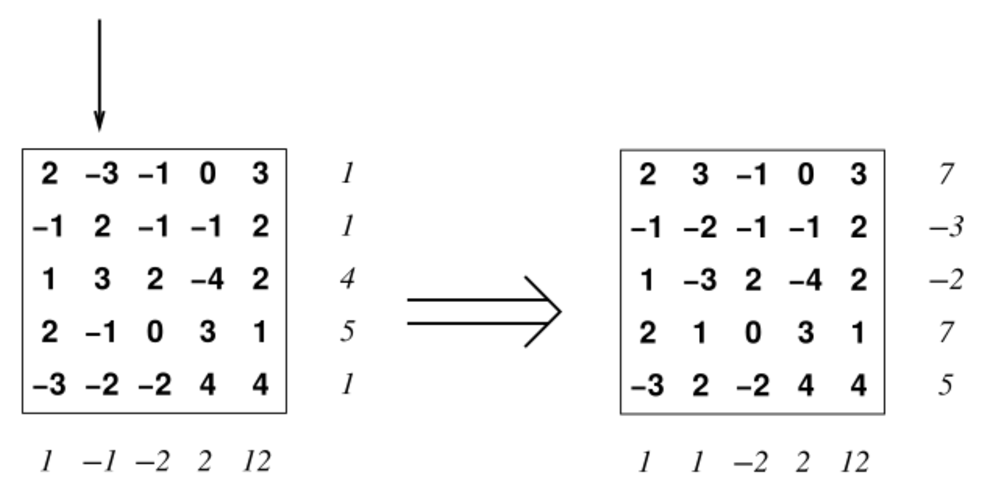
\includegraphics[scale=0.6]{Figs/Algorithms/array}
\end{figure}
\begin{enumerate}[(1)]
\item Существует (конечная) последовательность операций, которая приведёт к целевому положению.
\item Любая последовательность операций в конечном итоге достигнет целевого положения.
\item Каждая последовательность операций достигает цели за одинаковое число шагов.
\item Никакая последовательность операций не может достичь цели.
\end{enumerate}

Алгоритмические задачи обычно решаются нахождением параметра $P$ --- некоего числового показателя состояний, который каким-либо образом закрепляет прогресс продвижения к целевому состоянию.

Для доказательства (1), нужно показать, что до того, как вы достигнете целевого состояния, всегда будет существовать операция (или последовательность операций), улучшающая $P$.
Чтобы не попасть в ловушку парадокса Зенона (делая шаги всё меньше и меньше, и никогда не достигая цели), возможно, придётся доказать, что $P$ можно всегда улучшить, по крайней мере, на некоторую величину, или что существует только конечное число возможных позиций.

Для доказательства (2), вы делаете то же самое, но показываете, что \emph{любая} операция улучшает $P$.

Чтобы доказать (3), вы показываете, что каждая операция улучшает $P$ на одну и ту же величину.

Чтобы доказать (4), вы показываете, что \emph{не существует} операции, улучшающей $P$, а для достижения цели требуется улучшение.

\medskip

Вернёмся к задаче с таблицей.
Мы видим, что число линий (строк и столбцов) с неотрицательной суммой --- неправильный параметр.
Это число может уменьшаться даже тогда, когда линия с отрицательной суммой поменяла знак.
Вместо этого попробуем придать $P$ значение суммы всех чисел в таблице.
Перевернув строку с суммой $-S$, параметр $P$ увеличивается на $2S$, так как $P$ можно записать как сумму сумм всех строк (аналогично для столбцов).
Поскольку имеется только конечное число достижимых позиций
(а именно, не более, чем $2^{m+n}$), и $P$ растёт каждый раз, когда переворачивается линия с отрицательной суммой, то должен настать момент, когда сумма в каждой из линий неотрицательна.

Эта задача типа (1), но её можно также переформулировать как задачу типа (2).
Для этого следует добавить условие, что можно переворачивать только линии с отрицательными суммами, а затем потребовать доказать, что вы \emph{достигнете} такого момента, когда сумма в каждой линии неотрицательна.

\medskip

{
\sloppy

Задачи, приведённые ниже, могут потребовать значительно большей изобретательности для отыскания параметра $P$.

}

\subsection*{Инфекция на шахматной доске}% (THE INFECTED CHECKBOARD)
\rindex{Инфекция на шахматной доске}

Инфекция распространяется по клеткам шахматной доски $n \times n$ следующим образом: если у клетки два или более инфицированных соседа, то она также заражается.
(Соседями считаются только клетки с общей стороной, так что у каждой клетки имеется максимум четыре соседа.)

\begin{figure}[h!]
\centering
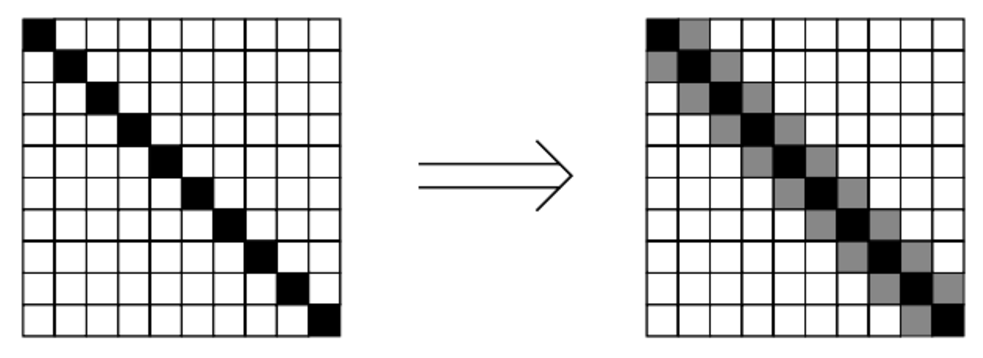
\includegraphics[scale=0.6]{Figs/Algorithms/diag}
\end{figure}

Предположим, например, что все $n$ клеток на главной диагонали инфицированы.
Тогда инфекция распространится на соседние диагонали и в итоге на всю доску.

Докажите, что нельзя заразить всю шахматную доску, если изначальное число инфицированных клеток меньше $n$.

\subsection*{Пустое ведро}% (EMPTYING A BUCKET)
\rindex{Пустое ведро}

Имеются три больших ведра, в каждом налито целое число унций жидкости.
В любой момент вы можете удвоить объём жидкости в одном из вёдер, долив туда из ведра с б\'{о}льшим объёмом жидкости.
Другими словами, разрешается переливать из ведра, содержащего $x$ унций жидкости в ведро, содержащее 
$y\le x$ унций, до тех пор, пока там не станет $2y$ унций (а в первом ведре останется $x-y$).

\begin{figure}[h!]
\centering
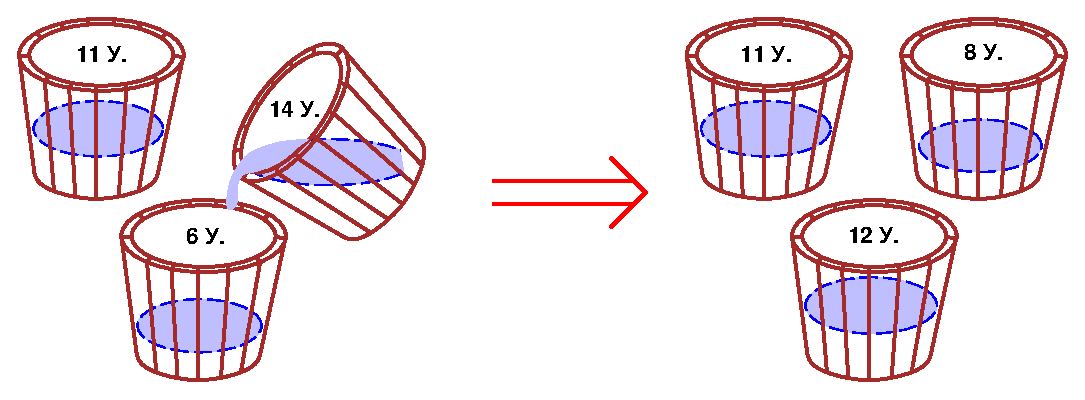
\includegraphics[scale=0.6]{Figs/Algorithms/buckets-ru}
\end{figure}

Докажите, что независимо от начального состояния, вы сможете вылить всю жидкость из одного из вёдер.

\subsection*{Фишки по углам}% (PEGS ON THE CORNERS)
\rindex{Фишки по углам}

Четыре фишки начинают ходить с углов некоего квадрата на плоскости.
В любой момент одна фишка может перепрыгнуть через другую,
встав на том же расстоянии с противоположной стороны.
Фишка, через которую перепрыгнули, остаётся на месте.
Возможно ли передвинуть все фишки так, чтобы они оказались в углах б\'{о}льшего квадрата?

\subsection*{Фишки на полуплоскости}% (PEGS ON THE HALF-PLANE)
\rindex{Фишки на полуплоскости}

В каждой вершине целочисленной решётки координатной плоскости, на оси $X$ и ниже неё стоит по фишке.
В любой момент фишка может перепрыгнуть через соседнюю с ней фишку (по горизонтали, вертикали или диагонали) и встать на следующую вершину решётки, при условии, что она не занята.
При этом фишка, через которую перепрыгнули, снимается с поля.

\begin{figure}[h!]
\centering
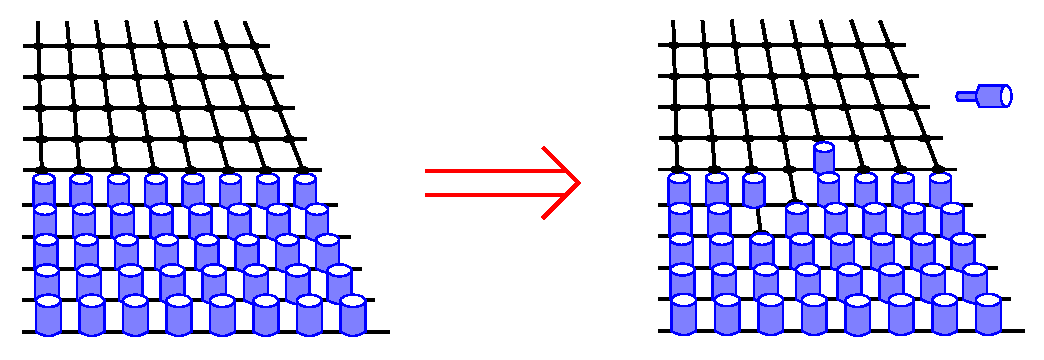
\includegraphics[scale=0.6]{Figs/Algorithms/pegs}
\end{figure}

Может ли фишка продвинуться произвольно далеко наверх от оси~$X$?

\subsection*{Фишки на квадрате}% (PEGS IN A SQUARE)
\rindex{Фишки на квадрате}

И снова фишки расположены в вершинах решётки на плоскости, только в этот раз в квадрате $n\times n$.
В данной задаче фишки могут прыгать только по горизонтали или вертикали, и фишка, через которую перепрыгнули, убирается с поля.
Цель задачи --- уменьшить число фишек с $n^2$ до $1$.

Докажите, что в случае, когда $n$ кратно $3$, этого сделать нельзя!

\subsection*{Кульбиты многоугольника}% (FLIPPING THE POLYGON)
\rindex{Кульбиты многоугольника}

Вершины многоугольника обозначены числами, сумма которых положительна.
В любой момент разрешается поменять знак у вершины с отрицательным числом, но тогда новое значение вычитается из обеих чисел, обозначающих соседние вершины, так чтобы сумма оставалась постоянной.

\begin{figure}[h!]
\centering
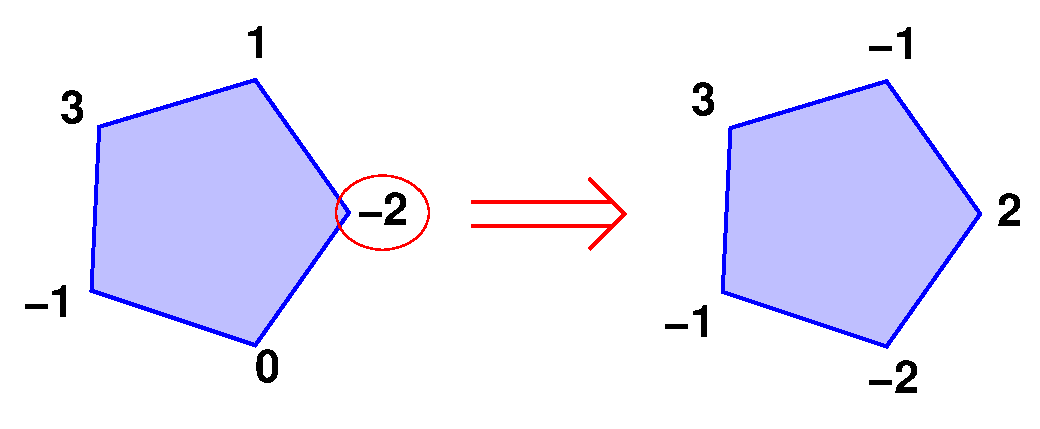
\includegraphics[scale=0.6]{Figs/Algorithms/pent}
\end{figure}

Докажите, что вне зависимости от порядка выбора чисел, после конечного числа шагов все числа окажутся положительными, и, таким образом, процесс прекратится.

\subsection*{Лампочки по кругу}% (LIGHT BULBS IN A CIRCLE)
\rindex{Лампочки по кругу}

Лампочки расставлены по кругу и пронумерованы от $1$ до $n$.
Изначально они все включены.
В момент времени $t$ вы смотрите на лампочку номер $t \pmod{n}$, и если она включена, то меняете состояние у лампочки $t + 1 \pmod{n}$;
то есть выключаете её, если она включена, и включаете, если она выключена.
Если лампочка $t$ выключена, то вы ничего не делаете.

Докажите, что если ходить и ходить по кругу подобным образом, то в конце концов наступит момент, когда все лампочки снова будут включены.

\subsection*{Жуки на многограннике}% (BUGS ON A POLYHEDRON)
\rindex{Жуки на многограннике}

На каждой грани выпуклого многогранника живёт по жуку.
Жуки ползают по периметру своей грани с разными скоростями, но только по часовой стрелке.
Докажите, что невозможно создать такое расписание, чтобы жуки могли обойти свою грань и вернуться к начальной точке, ни с кем не столкнувшись.

\subsection*{Жуки на числовом луче}% (BUGS ON THE LINE)
\rindex{Жуки на числовом луче}

В каждой положительной целочисленной точке на числовом луче стоит зелёная, жёлтая или красная лампочка.
Жук ставится на «1» и ползёт, подчиняясь следующим правилам:
\begin{itemize}
\item если он видит зелёный свет, он переключает его на жёлтый и передвигается на один шаг вправо; 
\item если он видит жёлтый свет, он переключает его на красный и передвигается на один шаг вправо; 
\item если же он видит красный свет, он переключает его на зелёный и передвигается на один шаг \emph{влево}.
\end{itemize}

В конце концов, жук либо свалится с левого конца луча, либо уползёт на бесконечность вправо.
Затем второй жук ставится на «1», затем третий.

Докажите, что если второй жук свалился с левого конца луча, то третий жук уползёт на бесконечность.

\subsection*{Как разломать шоколадку}% (BREAKING A CHOCOLATE BAR)
\rindex{Как разломать шоколадку}

Дана шоколадка из $m\times n$ квадратных долек. 
Требуется разломать её на составные дольки.
За один шаг вы можете взять один кусок и разломить его по вертикальной или горизонтальной линии.

Докажите, что какой бы вы метод ни выбрали, вам потребуется одно и то же  число шагов.

\begin{figure}[h!]
\centering
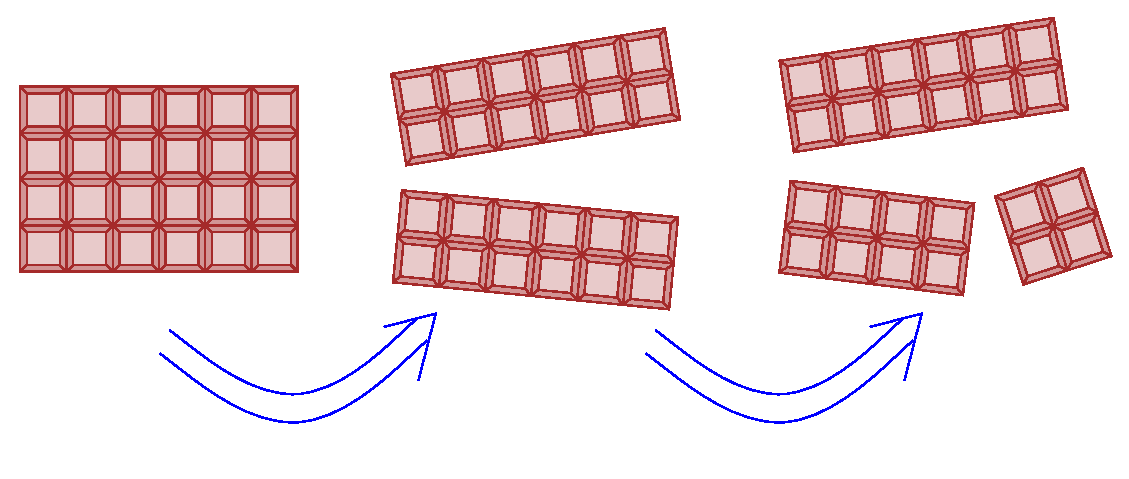
\includegraphics[scale=0.5]{Figs/Algorithms/bar}
\end{figure}
